\subsection{Friday, October 7: Cosets and Theorem of Lagrange}

\subsubsection{Cosets}

\begin{theorem}
    Let $G$ be a group and suppose $H \leq G$. Let the relation $\sim_L$ be defined on $G$ by $a \sim_L b \Leftrightarrow a^{-1}b \in H$ and let the relation $\sim_R$ be defined on $G$ by $a \sim_R b \Leftrightarrow ab^{-1} \in H$. Then $\sim_L$ and $\sim_R$ are both equivalence relations on $G$.
\end{theorem}

\begin{definition}
    Let $G$ be a gorup and suppose $H \leq G$. The subset
    \[ Ha = \qty{ha \mid h \in H} \]
    of $G$ is the \textbf{right coset of $H$ containing $a$} whit the set
    \[ aH = \qty{ah \mid h \in H} \]
    of $G$ is the \textbf{left coset of $H$ containing $a$}. In $aH$ or $Ha$, $a$ is called a \textbf{coset representative}. Any element of $aH$ or $Ha$ can be made a representative of the coset.
\end{definition}

\begin{exercise}
    Let $Q_8 = \qty{1, i, j, k, -1, -i, -j, -k}$ (\textbf{quaternion group}) with identity element 1 and noncummitative multiplication given by
    \[ \qty(-1)^2 = 1, i^2 = j^2 = k^2 = -1 \]
    \[ ij = -ji - k, jk= -kj = i, ki = -ik = j \]
    \[ -x = \qty(-1)x = x\qty(-1) \forall x \in Q_8 \]
    \begin{itemize}
        \item Find the center of this group
        \item Let $H = \qty{1, j, -1, -j}$. Find the left and right cosets of subgroup $H$ in $Q_8$
    \end{itemize}
\end{exercise}

\begin{solution}
    \begin{itemize}
        \item Note that we are looking for values in $Q_8$ that commutes with every element. Thus, $z\qty(Q_8) = \qty{z \in Q_8 \mid xz = zx \, \forall x \in Q_8} = \qty{1, -1}$.
        \item The left cosets of subgroup $H$ in $Q_8$ are
        \[ H = \qty(1)H = jH = \qty(-1)H = \qty(-j)H \]
        and
        \[ kH = \qty{k, -i, -k, i} = \qty(-i)H = \qty(-k)H = iH  \]
        So we have $H \cup kH = Q_8$.  
        \item The right cosets are 
        \[ H = H(1) = Hj = H(-1) = H(-j) \]
        and
        \[ Hi = \qty{i, -k, -i, k} = H \qty(-k) = H \qty(-i) = Hk \]
        So we have, $H \cup Hi = Q_8$.
    \end{itemize}
\end{solution}

\begin{exercise}
    Consider $\langle U \qty(\Z_{16}), \cdot_{16} \rangle$. Find the left cosets of the subgroups $\langle 7 \rangle$ and $\langle 11 \rangle$ in $U \qty(\Z_{16})$
\end{exercise}

\begin{solution}
    Note that $U \qty(Z_{16}) = \qty{1, 3, 5, 7, 9, 11, 13, 15}$. 
    \begin{itemize}
        \item For $\langle 7 \rangle$, we have
        \begin{align*}
            \langle 7 \rangle &= \qty{1, 7} = 1 \langle 7 \rangle = 7 \langle 7 \rangle \\
            3 \langle 7 \rangle &= \qty{3, 5} = 5 \langle 7 \rangle \\
            9 \langle 7 \rangle &= \qty{9, 15} = 15 \langle 7 \rangle \\
            11 \langle 7 \rangle &= \qty{11, 13} = 13 \langle 7 \rangle 
        \end{align*}
        So we have 4 left cosets of $\langle 7 \rangle$. Note that the right cosets are the same since the group is abelian.
        \item For $\langle 11 \rangle$
        \begin{align*}
            \langle 11 \rangle &= \qty{1, 11, 9,  3} \\
            5 \langle 11 \rangle &= \qty{5, 7, 13, 15} 
        \end{align*}
        So we have 2 left cosets of $\langle 11 \rangle$.
    \end{itemize}
\end{solution}

\begin{remark}
    Let $G$ be a group and $H \leq G$. \\
    \begin{enumerate}
        \item If $e \in G$ is the identity, $eH = H = He$
        \item For any $a \in G, a \in aH$
        \item Let $a, b \in G$ \\
        \begin{enumerate}[a.]
            \item $aH = bH \Leftrightarrow a^{-1}b \in H$
            \item $Ha = Hb \Leftrightarrow ab^{-1} \in H$
        \end{enumerate}
        \item Let $a \in G$ \\
        \begin{enumerate}
            \item $aH = H \Leftrightarrow a \in H$
            \item $Ha = H \Leftrightarrow a \in H$
        \end{enumerate}
        \item If $G$ is abelian, then $aH = Ha$. The converse is not necessarily true. That is, there exist subgroups $H$ for which $aH = Ha$, for all $a \in G$, even if $G$ is not abelian.
    \end{enumerate}
\end{remark}

\subsubsection{Theorem of Lagrange}

\begin{theorem}
    Let $G$ be a group and suppose $H \leq G$. Then for any $a \in G, \qty|H| = \qty|aH| = \qty|Ha|$.
\end{theorem}

\begin{theorem}[Lagrange]
    Let $G$ be a finite group and suppose $H \leq G$. Then $\qty|H|$ divides $\qty|G|$.
\end{theorem}

\begin{corollary}
    Let $G$ be a finite group with $\qty|G| = n$. Then, for any $a \in G$, $\qty|a|$ divides $n$ and $a^n  = e$.
\end{corollary}

\begin{exercise}
    Consider the dihedral group $D_{10}$ where $a^{10} = b^2 = \qty(ab)^2 = e$. Find the order of the element $ba^6b^{-1}a^{22}b^6$
\end{exercise}

\begin{solution}
    Note that $\qty|D_{10}| = 2 \cdot 10 = 20$ and $D_{10} = \langle a \rangle \cup \qty{a^kb \mid k = 0, 1, \ldots, 9}$. Moreover, $ba^k = a^{10 -k}b, k \in \Z^+$. Note that
    \[ ba^6b^{-1}a^{22}b^6 = a^4bba^2 = a^4a^2 = a^6 \]
    Therefore, $\qty|ba^6b^{-1}a^{22}b^6| = \qty|a^6| = \frac{10}{\text{gcd}\qty(10, 6)} = \frac{10}{2} = 5$
\end{solution}

\begin{corollary}
    Every group of prime order is cyclic.
\end{corollary}

\begin{definition}
    The number of distinct left cosets of $H$ in $G$ is called the \textbf{index of $H$ in $G$} and is denoted by $\qty[G : H].$
\end{definition}

\begin{remark}
    A subgroup with index 1 is the whole group.
\end{remark}

\begin{corollary}
    If $G$ is a finite group and $K \leq H \leq G$, then $\qty[G : K] = \qty[G : H] \cdot \qty[H : K]$
\end{corollary}

\begin{theorem}
    Let $H \leq G$. Then the number of left cosets of $H$ is equal to the number of right cosets of $H$ in $G$.
\end{theorem}

\begin{exercise}
    If $H$ and $K$ are subgroups of $G$ and $g \in G$, show that $g \qty(H \cap K) = gH \cap gK$
\end{exercise}

\begin{proof} \phantom{blank} \\
    $\qty(\subseteq)$ Let $gx \in g\qty(H \cap K)$. 
    \begin{align*}
        &\Rightarrow x \in H \cap K \\
        &\Rightarrow x \in H \land x \in K \\
        &\Rightarrow gx \in gH \land gx \in gK \\
        &\Rightarrow gx \in gH \cap gK
    \end{align*}
    
    $\qty(\supseteq)$ Let $gy \in gH \cap gK$.  
    \begin{align*}
        &\Rightarrow gy \in gH \land gy \in gK \\
        &\Rightarrow y \in H \land y \in K \\
        &\Rightarrow y \in H \cap K \\
        &\Rightarrow gy \in g\qty(G \cap K)
    \end{align*}
\end{proof}

\begin{exercise}
    Suppose $G$ is a finite group with $\qty|G| = n$ and $\text{gcd}(k,n) = 1$. If $g \in G$ and $g^k = e$, show that $g = e$.
\end{exercise}

\begin{proof}
    Note that $\qty|g|\mid n = \qty|G|$. Since $g^k = e$, $\qty|g| \mid k$. This means that $\qty|g|$ is a common divisor of $n \land k$. Therefore, $\qty|g| = 1$ since gcd$\qty(k, n)  = 1$. Therefore $g = e$. \qedsymbol
\end{proof}

\begin{exercise}
    Suppose that $K$ is a proper subgroup of $H$ and $H$ is a proper subgroup of $G$. If $\qty|K| = 40$ and $\qty|G| = 600$, what are the possible orders of $H$?
\end{exercise}

\begin{solution}
    By the theorem of Lagrange, we have $\qty|K| \mid \qty|H|$ and $\qty|H| \mid \qty|G|$. This implies that $40 \mid \qty|H|$ and $\qty|H| \mid 600$. Thus, there exists $k_1, k_2 \in \Z^+$ such that $\qty|H| = 40k_1$ and $600 = \qty|H|k_2$. Therefore, $600 = \qty|H|k_2 = 40k_1k_2 \Rightarrow k_1k_2 = 15$.
    
    \begin{myspace}
        \begin{enumerate}[label=\textbf{Case \arabic*:}]
            \item If $k_1 = 1$ and $k_2 = 15$, $\qty|H| = 40 k_1 = 40 \cdot 1 = 40 = \qty|K|$. This is not possible since $K$ is a proper subgroup of $H$.
            \item If $k_1 = 15$ and $k_2 = 1$, $\qty|H| = 40k_1 = 40 \cdot 15 = 400 = \qty|G|$. This is not possible since $H < G$. 
            \item If $k_1 = 5$ and $k_2 = 3$, $\qty|H| = 40k_1 = 40 \cdot 3 = 120$.
            \item If $k_1 = 3$ and $k_2 = 5$, $\qty|H| = 40k_1 = 40 \cdot 5 = 200$.
        \end{enumerate}
    \end{myspace}
    Therefore, $\qty|H| = 120 \text{ or } 200$. 
\end{solution}

\begin{exercise}
    Determine up to isomorphism all groups of order four.
\end{exercise}

\begin{solution}
    Let $G$ be a group with $\qty|G| = 4$.
    \begin{myspace}
        \begin{enumerate}[label=\textbf{Case \arabic*:}]
            \item $G$ is cyclic: $G = \langle a \rangle = \qty{e, a, a^2, a^3} \cong \Z_4, \exists a \in G$.
            \item $G$ is not cyclic. Therefore $G$ has no elements of order 4. Thus, $\forall x \in G, x \neq e, \qty|x| \mid \qty|G| = 4$, but $\qty|x| \neq 4$. So we only have $\qty|x| = 2$. Remember that this is isomorphic to $V_4$ (Klein-4). Up to isomorphism, there are only two groups of order 4. 
        \end{enumerate}
    \end{myspace}
\end{solution}

\begin{exercise}
    Sketch the lattice diagram of $U\qty(\Z_{16})$
\end{exercise}

\begin{solution}
     Since $\qty|U\qty(\Z_{16})| = 8$. If $H \leq U\qty(\Z_{16})$, then $\qty|H| = 1, 2, 4, \text{ or } 8$ by Lagrange theorem. We will see the subgroups generated by each element. Note that $\langle 1 \rangle  = \qty{1}$, $\langle 7 \rangle = \qty{1, 7}$, $\langle 11 \rangle  = \qty{1, 11, 9, 3} = \langle 3 \rangle \cong \Z_4$, $\langle 5 \rangle = \qty{1, 5, 9, 13} = \langle 13 \rangle \cong \Z_4$, $\langle 15 \rangle = \qty{1, 15}$, $\langle 9 \rangle = \qty{1, 9} $. The lattice diagram is shown below, \\
     
     \begin{center}
         
        \tikzset{every picture/.style={line width=0.75pt}} %set default line width to 0.75pt        
        
        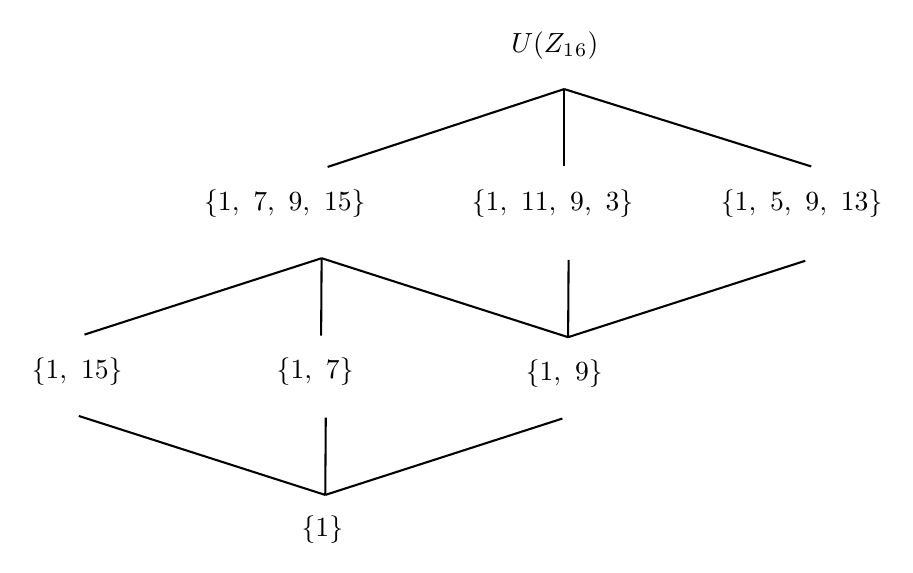
\begin{tikzpicture}[x=0.75pt,y=0.75pt,yscale=-1,xscale=1]
        %uncomment if require: \path (0,300); %set diagram left start at 0, and has height of 300
        
        %Straight Lines [id:da948235854717232] 
        \draw    (384,55.47) -- (270,93) ;
        %Straight Lines [id:da25429506457579265] 
        \draw    (503,92.75) -- (384,55.47) ;
        %Straight Lines [id:da7697582127285836] 
        \draw    (384,92.75) -- (384,55.47) ;
        %Straight Lines [id:da744451023155531] 
        \draw    (385.88,175.02) -- (500.12,138.22) ;
        %Straight Lines [id:da303229941938741] 
        \draw    (267.12,136.97) -- (385.88,175.02) ;
        %Straight Lines [id:da3001357018400008] 
        \draw    (386.12,137.74) -- (385.88,175.02) ;
        %Straight Lines [id:da17453134617677857] 
        \draw    (152.88,173.77) -- (267.12,136.97) ;
        %Straight Lines [id:da14293581086388807] 
        \draw    (267.12,136.97) -- (266.88,174.25) ;
        %Straight Lines [id:da8601923762400443] 
        \draw    (268.88,251.02) -- (383.12,214.22) ;
        %Straight Lines [id:da47520662968855176] 
        \draw    (150.12,212.97) -- (268.88,251.02) ;
        %Straight Lines [id:da7931296148316065] 
        \draw    (269.12,213.74) -- (268.88,251.02) ;
        
        % Text Node
        \draw (209,102.4) node [anchor=north west][inner sep=0.75pt]    {$\{1,\ 7,\ 9,\ 15\}$};
        % Text Node
        \draw (338,102.4) node [anchor=north west][inner sep=0.75pt]    {$\{1,\ 11,\ 9,\ 3\}$};
        % Text Node
        \draw (458,102.4) node [anchor=north west][inner sep=0.75pt]    {$\{1,\ 5,\ 9,\ 13\}$};
        % Text Node
        \draw (126,183.4) node [anchor=north west][inner sep=0.75pt]    {$\{1,\ 15\}$};
        % Text Node
        \draw (244,183.4) node [anchor=north west][inner sep=0.75pt]    {$\{1,\ 7\}$};
        % Text Node
        \draw (364,184.4) node [anchor=north west][inner sep=0.75pt]    {$\{1,\ 9\}$};
        % Text Node
        \draw (256,259.4) node [anchor=north west][inner sep=0.75pt]    {$\{1\}$};
        % Text Node
        \draw (357,26.4) node [anchor=north west][inner sep=0.75pt]    {$U(\mathbb{Z}_{1}{}_{6})$};
        
        \end{tikzpicture}

     \end{center}
\end{solution}